\chapter{DSOA}
\label{ch:3}
%TODO  todo introduzir capitulo

\section{Contexto e Motivação}
%TODO: Componentes baseados em serviços (limitações de cada 'mundo')


A natureza dinâmica e distribuída do ambiente SOA e o não-determinísmo dos atributos de qualidade sugere a necessidade de um sistema de monitoração contínua.

Nesse contexto, a plataforma DSOA estende as capacidades fornecidas pelas arquiteturas orientadas a componentes baseadas em serviços atuais, com a capacidade de adptação dos componentes em função dos atributos de qualidade.

Basicamente, um sistema de monitoração é composto por uma linguagem de especificação, um conjunto de sensores, analisadores e processadores de eventos.

[FIGURA MONITORAMENTO]



\section{Objetivo}
%TODO: objetivos DSOA

\section{Arquitetura}
\label{sec:dsoa_arch}

\begin{figure}[htp]
\centering
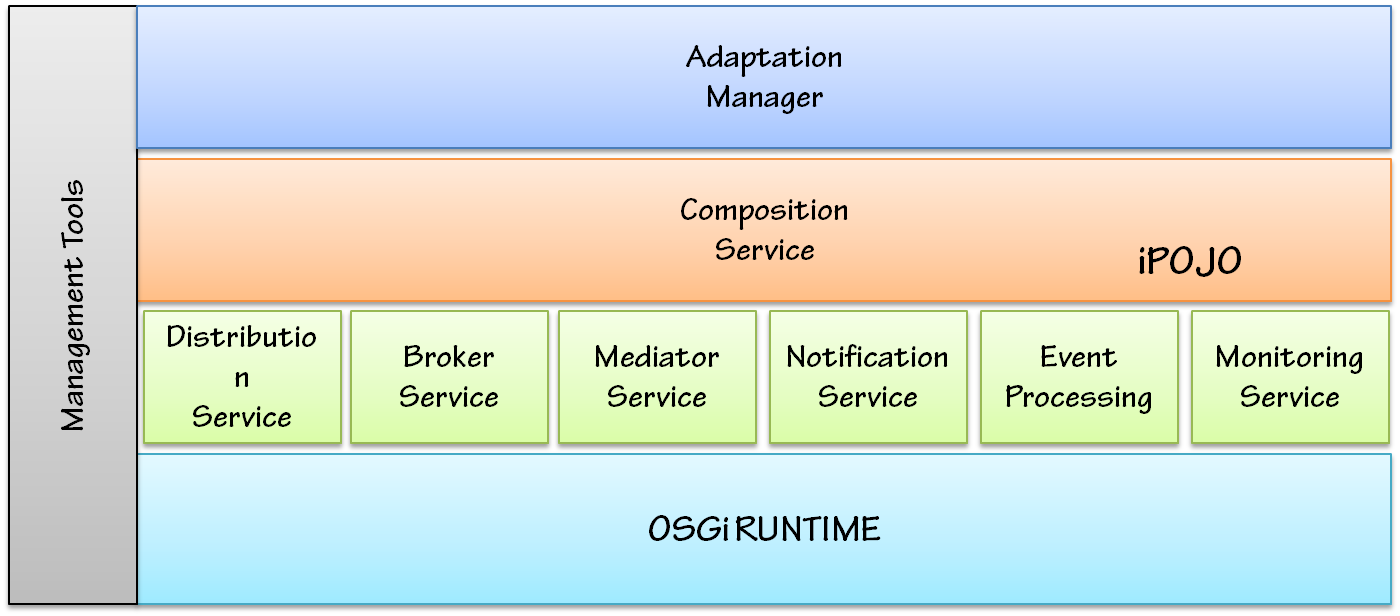
\includegraphics[width=13cm]{chapters/chapter3/dsoa-arch.png}
\caption[Arquitetura em Camdas DSOA]{Arquitetura em Camdas DSOA.}
\label{fig:proposal}
\end{figure}
%TODO arquitetura DSOA

\subsection{Componentes}
%TODO definir cada componente

\subsubsection{\textit{Distribution Service}}
%TODO

\subsubsection{\textit{Broker Service}}
%TODO

\subsubsection{\textit{Mediator Service}}
%TODO

\subsubsection{\textit{Notification Service}}
%TODO

\subsubsection{\textit{Event Processing Service}}
%TODO

\subsubsection{\textit{Monitoring Service}}
%TODO

\subsubsection{\textit{Composition Service}}
%TODO

\subsubsection{\textit{Adaptation Manager}}
%TODO

\subsubsection{\textit{Management Tool}}
%TODO


